\documentclass{beamer}
\usetheme{Madrid}
\usepackage{graphicx}
\usepackage{amsmath}
\usepackage{tikz}

\title[Modelamiento DES]{Modelamiento de la Planta Industrial mediante Sistemas de Eventos Discretos (DES)}
\author{Jorge Emilio Melo,Juan David Medina Pérez, Nicolás Arias}
\date{\today}

\begin{document}

%-------------------------------------------
\begin{frame}
\titlepage
\end{frame}

%-------------------------------------------
\begin{frame}{Planta Industrial Analizada}
La planta está compuesta por tres módulos principales:

\begin{itemize}
    \item Un \textbf{distribuidor rotativo (turntable)} que direcciona las piezas.
    \item Dos \textbf{células robot–máquina CNC}, cada una encargada de tomar piezas y ejecutar una operación.
    \item Una red de \textbf{transportadores} que conecta la entrada, distribución y salida.
\end{itemize}

\begin{center}
\includegraphics[width=0.8\textwidth]{Imagenes/PLANTA-TOTAL.png}
\end{center}

\end{frame}

%-------------------------------------------
\begin{frame}{Módulo 1 – Distribuidor Rotativo}
El distribuidor recibe piezas desde las bandas y las orienta hacia la estación apropiada.
\begin{columns}
    \column{0.48\textwidth}
    \begin{itemize}
    \item Estados principales:
    \begin{itemize}
        \item 1: Espera / mesa libre
        \item 2: Pieza proveniente de banda B
        \item 3: Pieza proveniente de banda G
        \item 4: Rotación hacia salida
        \item 5: Descarga y retorno
    \end{itemize}
    \end{itemize}
    \column{0.48\textwidth}
    \begin{center}
    \includegraphics[width=0.85\textwidth]{Imagenes/distribuidor-completo.png}
    \end{center}
\end{columns}
\end{frame}

%-------------------------------------------
\begin{frame}{Modelo DES del Distribuidor}
El automata asociado se describe mediante:

\[
\Sigma = \{B\_E, G\_E, ROT, UNLOAD, RESET\}
\]

\begin{center}
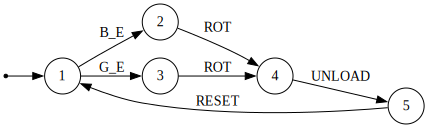
\includegraphics[width=0.55\textwidth]{Imagenes/graphviz-distri.png}
\end{center}

Este modelo captura:
\begin{itemize}
    \item Exclusión entre entradas.
    \item Secuencia de giro–descarga.
    \item Retorno automático al estado inicial.
\end{itemize}

\end{frame}

%-------------------------------------------
\begin{frame}{Módulo 2 – Células Robot–Máquina}
Cada célula está compuesta por:
\begin{itemize}
    \item Robot manipulador industrial.
    \item Máquina CNC cerrada.
    \item Interbloqueos de seguridad.
\end{itemize}

\begin{center}
\includegraphics[width=0.7\textwidth]{Imagenes/ENSAMBLADOR.png}
\end{center}

\end{frame}

%-------------------------------------------
\begin{frame}{Modelo DES de la Estación Robot–Máquina}

Estados simplificados:
\begin{itemize}
    \item 1: Espera de pieza
    \item 2: Robot toma material (E)
    \item 3: Robot entrega a máquina (F)
    \item 1: Retorno del robot (R)
\end{itemize}

\begin{center}
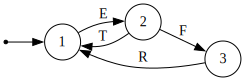
\includegraphics[width=0.56\textwidth]{Imagenes/graphviz-maquina.png}
\end{center}

El ciclo es síncrono con la mesa distribuidora y requiere supervisión para evitar colisiones lógicas.
\end{frame}
%-------------------------------------------
\begin{frame}{Requerimientos del Sistema}
Los requerimientos funcionales y de control que guiarán el diseño del supervisor son:

\textbf{1. Buffer}
\begin{itemize}
    \item Cada entrada del distribuidor contiene un buffer que almacene por lo menos 3 piezas que entrega la maquina.
\end{itemize}

\textbf{2. Mesa Distribuidora}
\begin{itemize}
    \item La distribuición de piezas debe ser rotativa entre cada una .
\end{itemize}
\end{frame}
\end{document}
